\section{Evaluación}

\subsection{Medida de Error}

Tanto para el caso de la segmentación de los vídeos como la reconstrucción de los marcadores, se tiene los verdaderos marcadores generados en la secuencia, por lo que es necesario establecer una medida de error sobre la salida de los algoritmos. Se eligió aplicar una metodología basada en la distancia euclidiana promedio, entre los marcadores de ambos conjuntos \cite{humaneva} . 

Asumiendo que los conjuntos de datos de salida de algoritmos y ground truth, tienen sus cuadros sincronizados temporalmente, en un cuadro [f] dado se tienen $M$ marcadores en un conjunto $ \boldsymbol{x},\quad\{m_{i}(x)\},i=1,\ldots,M $ , donde $ m_{i}(x)\in{\mathbf{R}^{3}} $ ( o $ \mathbf{R}^{2} $ para el caso de las vistas de cámaras individuales), y $ \boldsymbol{\tilde{x}} $ es el conjunto ground truth con la misma cantidad $M$ de marcadores alineados con $\boldsymbol{x}$ (el $i$-esimo marcador de $\boldsymbol{x}$ se corresponde con el  $i$-esimo marcador de $\boldsymbol{\tilde{x}}$), se calcula la distancia como

\begin{equation}
D(\boldsymbol{x_{f}},\boldsymbol{\tilde{x_{f}}})=\frac{1}{M}\sum_{i=1}^{M} \|m_{i}^{[f]}(\boldsymbol{x})-m_{i}^{[f]}(\boldsymbol{\tilde{x}})\|
\label{error_vs_ground_basica}
\end{equation}

Sin embargo, el calculo debe ser modificado para contemplar para el caso en que la cantidad de marcadores a la salida del procesamiento es menor a $M$, se define un conjunto binario en cada frame $\Delta=\{\delta_1,\delta_2,\ldots,\delta_M\}$, donde $\delta_i$ indica con 1 si el $i$-esimo marcador de $\boldsymbol{\tilde{x}}$ fue detectado, 0 en caso contrario. La ecuación \ref{error_vs_ground_basica} queda entonces

\begin{equation}
D(\boldsymbol{x_{f}},\boldsymbol{\tilde{x_{f}}},\Delta_{f})=\frac{1}{\sum_{j=1}^{M} \delta_j} \sum_{i=1}^{M} \delta_i.\|m_{i}^{[f]}(\boldsymbol{x})-m_{i}^{[f]}(\boldsymbol{\tilde{x}})\|
\label{error_vs_ground_deteccion}
\end{equation}

En una secuencia con $F$ frames, la performance promedio es calculada como el promedio de los errores en cada frame,

\begin{equation}
\mu_{secuencia} = \frac{1}{F}\sum_{f=1}^{F} D(\boldsymbol{x_{f}},\boldsymbol{\tilde{x_{f}}},\Delta_{f})
\label{performance_secuencia}
\end{equation}

Para poder trabajar con los datos a la salida de la segmentación y reconstrucción de las secuencias, es necesario obtener datos adicionales y entonces aplicar la ecuación \ref{performance_secuencia}. Específicamente, las parejas entre marcadores obtenidos y aquellos en el ground truth , que permite alinear y comparar los marcadores, y definir cuales fueron detectados.

El emparejamiento es realizado frame a frame, calculando en una matriz la distancia euclidiana entre todos los pares $\{i,j\}$, donde $i=1,\ldots,M_{x}$ es un marcador del conjunto $\boldsymbol{x}$ obtenido mediante algoritmo en un frame [f], y $j=1,\ldots,M_{\tilde{x}}$ es un marcador del conjunto $\boldsymbol{\tilde{x}}$ de ground truth,

\begin{equation}
d_{i,j}^{[f]} = \{\|m_{i}^{[f]}(\boldsymbol{x})-|m_{j}^{[f]}(\boldsymbol{\tilde{x}})\|\}
\label{distancia_algoritmo_ground}
\end{equation}

Una vez calculadas todas las distancias para un frame, se buscan aquellas parejas que presenta la menor distancia, relevando la pareja $(i,j)$  para la cual se verifica. Una vez obtenida esta distancia, los marcadores $(i,j)$ quedan descartados de la matriz, volviendo a buscar la siguiente pareja con distancia mínima, hasta que ya no queden elementos para emparejar (lo cual sucede en caso que se generen menos marcadores que en el ground truth como puede suceder en segmentación, o si todos los marcadores de ground truth ya fueron emparejados y sobran marcadores, como sucede en reconstrucción). Trabajar con las parejas en todos los grames de la secuencia, es análogo a trabajar con la ecuación (\ref{error_vs_ground_deteccion}) .

\subsection{Performance}

\subsubsection{Capturas Sintéticas}

Las multiples secuencias sinteticas generadas en Blender como fue establecido en (??? REFERENCIA BASE DE DATOS) son ingresadas al sistema, utilizando los parametros de calibracion de las camaras simuladas y los videos generados para las 17 camaras. Cada conjunto de datos fue procesado por cada uno de los bloques establecidos en ( ??? REFERENCIA BLOQUES SISTEMA COMPLETO) y comparado con el ground truth obtenido por Blender junto a los videos utilizando la metodologia establecida en ( ??? REFERENCIA MEDIDA ERROR ) para medir los resultados a la salida de cada bloque. Se realizaron las pruebas para 5 secuencias, 2 de las cuales fueron probadas con distinta adquisicion, indicadas en la tabla \ref{resultados_distintas_capturas} como $X,YY,Z$ donde $Z=1,2$ corresponden a dos tasas de muestreo diferentes.

\begin{table}[h]
\centering
\begin{tabular}{cccc|c|c|c|c|c|c|ll}
\cline{5-10}
& & & & SEGM. & SEGM. & RECONS. & RECONS. & TRACK. & TRACK. &  &  \\ \cline{1-10}
\multicolumn{1}{|c|}{captura} & \multicolumn{1}{c|}{markers} & \multicolumn{1}{c|}{frames} & n.cams & \begin{tabular}[c]{@{}c@{}}Promedio\\ (px)\end{tabular} & \begin{tabular}[c]{@{}c@{}}99\%\\ (px)\end{tabular} & \begin{tabular}[c]{@{}c@{}}Promedio\\ (cm)\end{tabular} & \begin{tabular}[c]{@{}c@{}}99\%\\ (cm)\end{tabular} & \begin{tabular}[c]{@{}c@{}}Promedio\\ (cm)\end{tabular} & \begin{tabular}[c]{@{}c@{}}99\%\\ (cm)\end{tabular} &  &  \\ \cline{1-10}
\multicolumn{1}{|c|}{8,03,1}  & \multicolumn{1}{c|}{14}         & \multicolumn{1}{c|}{89}     & 17      & 1,1063 & 3,6783  & 0,40778     & 2,6384  & 0,4318 & 2,9039  &  &  \\ \cline{1-10}
\multicolumn{1}{|c|}{8,07,1}  & \multicolumn{1}{c|}{14}         & \multicolumn{1}{c|}{62}     & 17      & 1,0871 & 3,1172  & 0,34382     & 1,806   & 0,34451     & 1,806   &  &  \\ \cline{1-10}
\multicolumn{1}{|c|}{8,07,2}  & \multicolumn{1}{c|}{14}         & \multicolumn{1}{c|}{123}    & 17      & 1,0912 & 3,3097  & 0,38736     & 1,2681
& 0,36381     & 1,2681  &  &  \\ \cline{1-10}
\multicolumn{1}{|c|}{8,11}    & \multicolumn{1}{c|}{13}         & \multicolumn{1}{c|}{94}     & 17      & 1,074  & 2,9042  & 0,38836     & 2,8705  & 0,38836     & 2,8705  &  &  \\ \cline{1-10}
\multicolumn{1}{|c|}{9,07,1}  & \multicolumn{1}{c|}{14}         & \multicolumn{1}{c|}{29}     & 17      & 1,1285 & 3,3211  & 0,28016     & 2,0401  & 0,28016     & 2,0401  &  &  \\ \cline{1-10}
\multicolumn{1}{|c|}{9,07,2}  & \multicolumn{1}{c|}{14}         & \multicolumn{1}{c|}{57}     & 17      & 1,1404 & 3,4476  & 0,34517     & 1,9902  & 0,34517     & 1,9902  &  &  \\ \cline{1-10}
\multicolumn{1}{|c|}{9,12,1}  & \multicolumn{1}{c|}{13}         & \multicolumn{1}{c|}{300}    & 15      & 1,0443 & 2,118   & 0,39731     & 1,4952  & 0,39741     & 1,4952  &  &  \\ \cline{1-10}
\end{tabular}
\caption{Resultados de los bloques, para distintas capturas sintéticas}
\label{resultados_distintas_capturas}
\end{table}

Los resultados para 17 camaras arrojan resultados similares en distintas capturas para el caso de amplia disponibilidad de camaras, y confirman los resultados y rendimientos presentados para los distintos bloques en las hipotesis planteadas para las capturas sinteticas. La segmentacion de los videos presenta errores promedios alrededor del pixel y errores maximos del entorno de los 4 pixeles. La reconstruccion y el tracking presentan resultados similares, siendo la diferencia conceptual entre ambas el etiquetado de trayectorias, y presentan resultados con error medio menor a los 0.5 cm, y errores maximos por debajo de 5 cm para el caso de reconstruccion con 17 camaras, y exceso de marcadores en reconstruccion (se establece como parametro de puntos reconstruidos una cantidad mayor a la esperada) 

\subsubsection{Ruido En Segmentación}

La prueba consiste en relevar el error promedio en reconstruccion, contra el ground truth 3D para distintas instancias de informacion de multiples vistas bajo ruido aleatorio de distintas magnitudes en pixeles en las coordenadas $X,Y$. Recordando que la diferencia entre las proyecciones 2D y los videos segmentados, son la visibilidad de los marcadores estimada en un 70\% por camara y el error de segmentacion estimada en 1 pixel, el ruido es inyectado entre la segmentacion y la reconstuccion siendo evaluada la salida de reconstrucción contra el ground truth 3D con el procedimiento de (??? REFERENCIA MEDIDA ERROR ) 

\begin{table}[h]
\centering
\begin{tabular}{|c|c|c|c|c|c|}
\hline
\textbf{Caso} & \textbf{\begin{tabular}[c]{@{}c@{}}Ruido\\ (px)\end{tabular}} & \textbf{\begin{tabular}[c]{@{}c@{}}14\\ Reconstr.\end{tabular}} & \textbf{\begin{tabular}[c]{@{}c@{}}18\\ Reconstr.\end{tabular}} & \textbf{\begin{tabular}[c]{@{}c@{}}30\\ Reconstr.\end{tabular}} & \textbf{\begin{tabular}[c]{@{}c@{}}46\\ Reconstr.\end{tabular}} \\ \hline
Ground Cam    & 0 & 7,84E-07       & 7,84E-07       & 7,84E-07       & 7,84E-07       \\ \hline
Segmentación  & 0 & 1,5792         & 0,38556        & 0,38556        & 0,38556        \\ \hline
Ground Cam    & 0,5          & 4,0817         & 0,45675        & 0,4453         & 0,42607        \\ \hline
Segmentación  & 0,5          & 13,6991        & 0,61128        & 0,61381        & 0,60517        \\ \hline
Ground Cam    & 1 & 16,9275        & 0,82309        & 0,72011        & 0,73301        \\ \hline
Segmentación  & 1 & 11,0847        & 0,8557         & 0,82286        & 0,83073        \\ \hline
Ground Cam    & 2 & 19,7131        & 1,7649         & 1,2152         & 1,2027         \\ \hline
Segmentación  & 2 & 15,9698        & 1,9701         & 1,3021         & 1,2884         \\ \hline
Ground Cam    & 4 & 28,6943        & 6,1386         & 2,1877         & 2,0468         \\ \hline
Segmentación  & 4 & 51,4025        & 5,7738         & 2,1484         & 2,1335         \\ \hline
Ground Cam    & 8 & 53,9555        & 14,3684        & 5,4929         & 3,8377         \\ \hline
Segmentación  & 8 & 264,8935       & 13,1539        & 4,7142         & 3,7993         \\ \hline
\end{tabular}
\caption{Resultados de Error Promedio (cm) en reconstrucción, para distintos caso de ruido en la segmentación, tanto resultados sobre vídeos como sobre ground truth}
\end{table}

Mas ruido implica mas incertidumbre en la reconstrucción, mientras mas ruidos, mas marcadores reconstruidos se precisan en reconstrucción para compensar la precision. Para mayor cantidad de marcadores en reconstrucción, se hace inviable la identificación de marcadores en tracking ?

\subsubsection{Variación Cantidad de Cámaras}

Reconstrucción con menos cámaras

Con menos cámaras, según que movimiento se está capturando indica que marcadores se ven afectados en reconstrucción

\begin{table}[h]
\centering
\begin{tabular}{|c|l|}
\hline
\textbf{CONJUNTO} & \multicolumn{1}{c|}{\textbf{CAMARAS}} \\ \hline
C17 & 1,2,3,4,5,6,7,8,9,10,11,12,13,14,15,16,17 \\ \hline
C15 & 3,4,5,6,7,8,9,11,12,13,14,15,16,17 \\ \hline
C8 & 3,5,7,9,11,13,15,17 \\ \hline
C6.1 & 4,6,8,12,14,16 \\ \hline
C6.2 & 3,6,9,11,14,17 \\ \hline
C6.3 & 3,5,9,11,13,17 \\ \hline
C6.4 & 3,7,9,11,15,17 \\ \hline
C5.1 & 1,3,9,11,17 \\ \hline
C5.2 & 1,4,8,12,16 \\ \hline
C4.1 & 4,8,12,16 \\ \hline
C4.2 & 3,9,11,17 \\ \hline
\end{tabular}
\caption{Distintas Combinaciones de Camaras del laboratorio sintetico, numeradas segun la figura \ref{img_espacio_capura} }
\end{table}

\begin{itemize}

\item Captura de Marcha, 8\_07\_100\_200

\begin{table}[h]
\centering
\begin{tabular}{c|c|c|c|c|c|}
\cline{2-6}
\textbf{} & \textbf{CONJUNTO} & \multicolumn{2}{c|}{\textbf{C17}} & \multicolumn{2}{c|}{\textbf{C8}} \\ \hline
\multicolumn{1}{|c|}{\textbf{MARKER}} & \textbf{NOMBRE} & \textbf{\begin{tabular}[c]{@{}c@{}}Promedio\\ (cm)\end{tabular}} & \textbf{\begin{tabular}[c]{@{}c@{}}99\%\\ (cm)\end{tabular}} & \textbf{\begin{tabular}[c]{@{}c@{}}Promedio\\ (cm)\end{tabular}} & \textbf{\begin{tabular}[c]{@{}c@{}}99\%\\ (cm)\end{tabular}} \\ \hline
\multicolumn{1}{|c|}{1} & LeftUpLeg & 0,3671 & 0,5158 & 0,3551 & 0,6197 \\ \hline
\multicolumn{1}{|c|}{2} & LeftLeg & 0,367 & 0,5411 & 0,3491 & 0,4464 \\ \hline
\multicolumn{1}{|c|}{3} & LeftFoot & 0,372 & 0,558 & 0,3582 & 0,5339 \\ \hline
\multicolumn{1}{|c|}{4} & RightUpLeg & 0,3714 & 0,5879 & 0,368 & 0,6825 \\ \hline
\multicolumn{1}{|c|}{5} & RightLeg & 0,378 & 0,586 & 0,3627 & 0,6065 \\ \hline
\multicolumn{1}{|c|}{6} & RightFoot & 0,4212 & 1,8483 & 0,3597 & 0,5667 \\ \hline
\multicolumn{1}{|c|}{7} & Spine & 0,404 & 0,6043 & 0,3819 & 0,5122 \\ \hline
\multicolumn{1}{|c|}{8} & Head & 0,3867 & 0,9063 & 0,3676 & 0,5208 \\ \hline
\multicolumn{1}{|c|}{9} & LeftArm & 0,3666 & 0,7997 & 0,3607 & 0,516 \\ \hline
\multicolumn{1}{|c|}{10} & LeftForeArm & 0,3873 & 0,9056 & 0,3621 & 0,6793 \\ \hline
\multicolumn{1}{|c|}{11} & LeftHand & 0,4007 & 1,1722 & 0,3667 & 0,7895 \\ \hline
\multicolumn{1}{|c|}{12} & RightArm & 0,4025 & 1,4771 & 0,3602 & 0,5078 \\ \hline
\multicolumn{1}{|c|}{13} & RightForeArm & 0,3844 & 0,781 & 0,36 & 0,5199 \\ \hline
\multicolumn{1}{|c|}{14} & RightHand & 0,3816 & 0,7728 & 0,3637 & 0,4884 \\ \hline
\multicolumn{1}{|c|}{\textbf{}} & \textbf{Secuencia} & \textbf{0,35686} & \textbf{0,81266} & \textbf{0,33603} & \textbf{0,53412} \\ \hline
\end{tabular}
\end{table}

\begin{table}[h]
\centering
\begin{tabular}{c|c|c|c|c|c|}
\cline{2-6}
\textbf{} & \textbf{CONJUNTO} & \multicolumn{2}{c|}{\textbf{C6.1}} & \multicolumn{2}{c|}{\textbf{C6.2}} \\ \hline
\multicolumn{1}{|c|}{\textbf{MARKER}} & \textbf{NOMBRE} & \textbf{\begin{tabular}[c]{@{}c@{}}Promedio\\ (cm)\end{tabular}} & \textbf{\begin{tabular}[c]{@{}c@{}}99\%\\ (cm)\end{tabular}} & \textbf{\begin{tabular}[c]{@{}c@{}}Promedio\\ (cm)\end{tabular}} & \textbf{\begin{tabular}[c]{@{}c@{}}99\%\\ cm)\end{tabular}} \\ \hline
\multicolumn{1}{|c|}{1} & LeftUpLeg & 5,821 & 37,6612 & 3,6182 & 45,3281 \\ \hline
\multicolumn{1}{|c|}{2} & LeftLeg & 0,3513 & 0,816 & PERDIDO & PERDIDO \\ \hline
\multicolumn{1}{|c|}{3} & LeftFoot & 0,3605 & 1,2945 & 0,3667 & 0,8624 \\ \hline
\multicolumn{1}{|c|}{4} & RightUpLeg & 4,1048 & 58,1895 & 1,2155 & 27,1109 \\ \hline
\multicolumn{1}{|c|}{5} & RightLeg & 0,3472 & 0,4227 & 0,3412 & 0,41 \\ \hline
\multicolumn{1}{|c|}{6} & RightFoot & 0,5627 & 9,3183 & 0,7806 & 19,5713 \\ \hline
\multicolumn{1}{|c|}{7} & Spine & 0,664 & 17,1032 & 0,4985 & 5,5806 \\ \hline
\multicolumn{1}{|c|}{8} & Head & 0,3559 & 0,4546 & 0,38 & 0,54 \\ \hline
\multicolumn{1}{|c|}{9} & LeftArm & 0,5959 & 6,4694 & 0,6544 & 9,2929 \\ \hline
\multicolumn{1}{|c|}{10} & LeftForeArm & 0,3472 & 0,4888 & 0,3608 & 0,656 \\ \hline
\multicolumn{1}{|c|}{11} & LeftHand & 0,3519 & 0,6833 & 0,3717 & 0,7004 \\ \hline
\multicolumn{1}{|c|}{12} & RightArm & 0,5879 & 6,7102 & 0,5145 & 9,4856 \\ \hline
\multicolumn{1}{|c|}{13} & RightForeArm & 0,3511 & 0,6307 & 0,3653 & 0,6726 \\ \hline
\multicolumn{1}{|c|}{14} & RightHand & 0,4799 & 7,4024 & 0,6051 & 14,0673 \\ \hline
 & \textbf{Secuencia} & \textbf{1,0095} & \textbf{24,3404} & \textbf{0,71806} & \textbf{17,1131} \\ \cline{2-6} 
\end{tabular}
\end{table}

\begin{table}[h]
\centering
\begin{tabular}{c|c|c|c|c|c|}
\cline{2-6}
\textbf{} & \textbf{CONJUNTO} & \multicolumn{2}{c|}{\textbf{C6.3}} & \multicolumn{2}{c|}{\textbf{C6.4}} \\ \hline
\multicolumn{1}{|c|}{\textbf{MARKER}} & \textbf{NOMBRE} & \textbf{\begin{tabular}[c]{@{}c@{}}Promedio\\ (cm)\end{tabular}} & \textbf{\begin{tabular}[c]{@{}c@{}}99\%\\ (cm)\end{tabular}} & \textbf{\begin{tabular}[c]{@{}c@{}}Promedio\\ (cm)\end{tabular}} & \textbf{\begin{tabular}[c]{@{}c@{}}99\%\\ (cm)\end{tabular}} \\ \hline
\multicolumn{1}{|c|}{1} & LeftUpLeg & 1,4455 & 22,4893 & PERDIDO & PERDIDO \\ \hline
\multicolumn{1}{|c|}{2} & LeftLeg & 0,3948 & 1,7799 & 0,5296 & 2,74 \\ \hline
\multicolumn{1}{|c|}{3} & LeftFoot & 0,3824 & 0,8816 & 0,3844 & 0,8658 \\ \hline
\multicolumn{1}{|c|}{4} & RightUpLeg & 1,1137 & 12,3685 & 1,4861 & 15,8273 \\ \hline
\multicolumn{1}{|c|}{5} & RightLeg & 0,4018 & 1,5785 & 0,3846 & 0,6913 \\ \hline
\multicolumn{1}{|c|}{6} & RightFoot & 0,3969 & 1,2771 & 0,393 & 1,3017 \\ \hline
\multicolumn{1}{|c|}{7} & Spine & 0,4152 & 1,4769 & 1,2313 & 10,2902 \\ \hline
\multicolumn{1}{|c|}{8} & Head & 0,384 & 0,7113 & 0,384 & 0,6934 \\ \hline
\multicolumn{1}{|c|}{9} & LeftArm & 0,5909 & 7,9405 & 0,3908 & 0,8389 \\ \hline
\multicolumn{1}{|c|}{10} & LeftForeArm & 0,4258 & 1,7149 & 0,3895 & 0,9638 \\ \hline
\multicolumn{1}{|c|}{11} & LeftHand & 0,3909 & 1,2141 & 0,3756 & 1,0439 \\ \hline
\multicolumn{1}{|c|}{12} & RightArm & 0,3756 & 0,7621 & 0,386 & 0,8189 \\ \hline
\multicolumn{1}{|c|}{13} & RightForeArm & 0,3968 & 0,9704 & 0,516 & 5,8124 \\ \hline
\multicolumn{1}{|c|}{14} & RightHand & 0,617 & 14,0623 & 0,7186 & 11,8042 \\ \hline
 & \textbf{Secuencia} & \textbf{0,51182} & \textbf{6,9322} & \textbf{0,5512} & \textbf{7,4726} \\ \cline{2-6} 
\end{tabular}
\end{table}

\begin{table}[h]
\centering
\begin{tabular}{c|c|c|c|c|c|}
\cline{2-6}
\textbf{} & \textbf{CONJUNTO} & \textbf{C5.1} & \textbf{C5.1} & \textbf{C5.2} & \textbf{C5.2} \\ \hline
\multicolumn{1}{|c|}{\textbf{MARKER}} & \textbf{NOMBRE} & \textbf{\begin{tabular}[c]{@{}c@{}}Promedio\\ (cm)\end{tabular}} & \textbf{\begin{tabular}[c]{@{}c@{}}99\%\\ (cm)\end{tabular}} & \textbf{\begin{tabular}[c]{@{}c@{}}Promedio\\ (cm)\end{tabular}} & \textbf{\begin{tabular}[c]{@{}c@{}}99\%\\ (cm)\end{tabular}} \\ \hline
\multicolumn{1}{|c|}{1} & LeftUpLeg & PERDIDO & PERDIDO & PERDIDO & PERDIDO \\ \hline
\multicolumn{1}{|c|}{2} & LeftLeg & 0,4295 & 2,3917 & 0,8971 & 22,988 \\ \hline
\multicolumn{1}{|c|}{3} & LeftFoot & 0,4147 & 0,7458 & 0,5518 & 8,6042 \\ \hline
\multicolumn{1}{|c|}{4} & RightUpLeg & 4,2922 & 58,0209 & PERDIDO & PERDIDO \\ \hline
\multicolumn{1}{|c|}{5} & RightLeg & 3,3777 & 61,5332 & 0,3934 & 1,5824 \\ \hline
\multicolumn{1}{|c|}{6} & RightFoot & PERDIDO & PERDIDO & 0,493 & 4,8055 \\ \hline
\multicolumn{1}{|c|}{7} & Spine & 18,9827 & 50,6854 & 16,6915 & 35,0544 \\ \hline
\multicolumn{1}{|c|}{8} & Head & 9,2659 & 22,7929 & PERDIDO & PERDIDO \\ \hline
\multicolumn{1}{|c|}{9} & LeftArm & 0,5064 & 4,9531 & 0,3648 & 0,5347 \\ \hline
\multicolumn{1}{|c|}{10} & LeftForeArm & 0,6575 & 10,2007 & 0,7586 & 13,8037 \\ \hline
\multicolumn{1}{|c|}{11} & LeftHand & 0,6831 & 13,8355 & 1,5395 & 25,0238 \\ \hline
\multicolumn{1}{|c|}{12} & RightArm & 0,7107 & 14,7915 & 0,6703 & 7,409 \\ \hline
\multicolumn{1}{|c|}{13} & RightForeArm & 2,3882 & 34,3833 & PERDIDO & PERDIDO \\ \hline
\multicolumn{1}{|c|}{14} & RightHand & 1,906 & 38,9179 & PERDIDO & PERDIDO \\ \hline
 & \textbf{Secuencia} & \textbf{3,0121} & \textbf{40,035} & \textbf{1,0513} & \textbf{20,5912} \\ \cline{2-6} 
\end{tabular}
\end{table}

\begin{table}[h]
\centering
\begin{tabular}{c|c|c|c|c|c|}
\cline{2-6}
\textbf{} & \textbf{CONJUNTO} & \multicolumn{2}{c|}{\textbf{C4.1}} & \multicolumn{2}{c|}{\textbf{C4.2}} \\ \hline
\multicolumn{1}{|c|}{\textbf{MARKER}} & \textbf{NOMBRE} & \textbf{\begin{tabular}[c]{@{}c@{}}Promedio\\ (cm)\end{tabular}} & \textbf{\begin{tabular}[c]{@{}c@{}}99\%\\ (cm)\end{tabular}} & \textbf{\begin{tabular}[c]{@{}c@{}}Promedio\\ (cm)\end{tabular}} & \textbf{\begin{tabular}[c]{@{}c@{}}99\%\\ (cm)\end{tabular}} \\ \hline
\multicolumn{1}{|c|}{1} & LeftUpLeg & PERDIDO & PERDIDO & 2,167 & 31,4114 \\ \hline
\multicolumn{1}{|c|}{2} & LeftLeg & 0,565 & 9,7164 & 1,1854 & 26,0476 \\ \hline
\multicolumn{1}{|c|}{3} & LeftFoot & 0,38 & 0,9696 & 0,4273 & 0,7269 \\ \hline
\multicolumn{1}{|c|}{4} & RightUpLeg & PERDIDO & PERDIDO & 0,8181 & 13,8336 \\ \hline
\multicolumn{1}{|c|}{5} & RightLeg & 0,6517 & 13,5 & PERDIDO & PERDIDO \\ \hline
\multicolumn{1}{|c|}{6} & RightFoot & 0,4682 & 4,8055 & 0,4841 & 1,1391 \\ \hline
\multicolumn{1}{|c|}{7} & Spine & 3,1591 & 30,8635 & 3,7266 & 29,8362 \\ \hline
\multicolumn{1}{|c|}{8} & Head & 0,3595 & 0,4278 & 0,388 & 0,54 \\ \hline
\multicolumn{1}{|c|}{9} & LeftArm & 0,3609 & 0,5417 & 0,4155 & 0,5588 \\ \hline
\multicolumn{1}{|c|}{10} & LeftForeArm & 2,8277 & 25,0512 & 2,8636 & 17,1966 \\ \hline
\multicolumn{1}{|c|}{11} & LeftHand & 0,6116 & 9,755 & 0,4814 & 3,8581 \\ \hline
\multicolumn{1}{|c|}{12} & RightArm & 0,6862 & 11,1969 & 0,6188 & 12,4351 \\ \hline
\multicolumn{1}{|c|}{13} & RightForeArm & 2,0736 & 21,7146 & 2,2073 & 25,8873 \\ \hline
\multicolumn{1}{|c|}{14} & RightHand & 0,9646 & 22,845 & PERDIDO & PERDIDO \\ \hline
 & \textbf{Secuencia} & \textbf{1,3662} & \textbf{23,0206} & \textbf{1,1976} & \textbf{22,5326} \\ \cline{2-6} 
\end{tabular}
\end{table}

\item Captura de Movimiento Libre, 9\_12\_100\_100

\begin{figure}[H]
  \centering
   \subfloat[Trayectorias Movimiento Libre.]{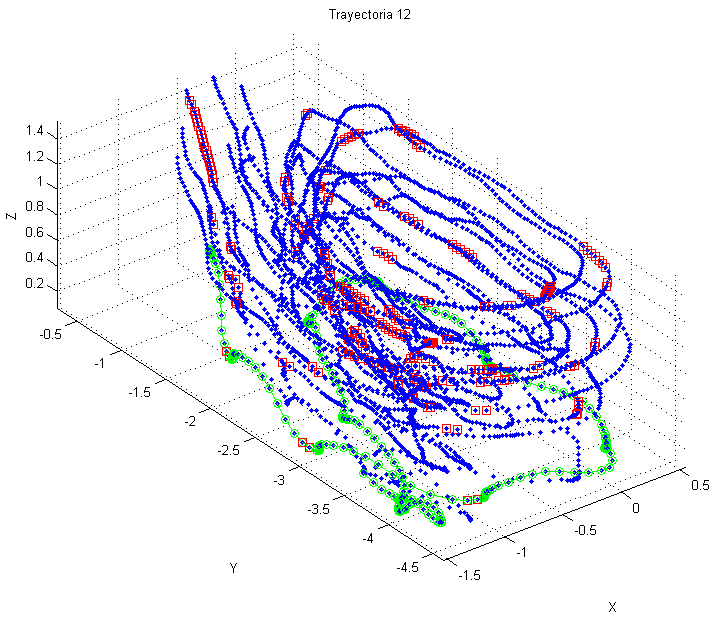
\includegraphics[scale=0.4]{img/Performance/00_Trayectorias_Tracking.png}\label{tracking_movimiento_libre}}\hspace{3 mm}
   \subfloat[Trayectoria Marcador, y Esqueleto reconstruido.]{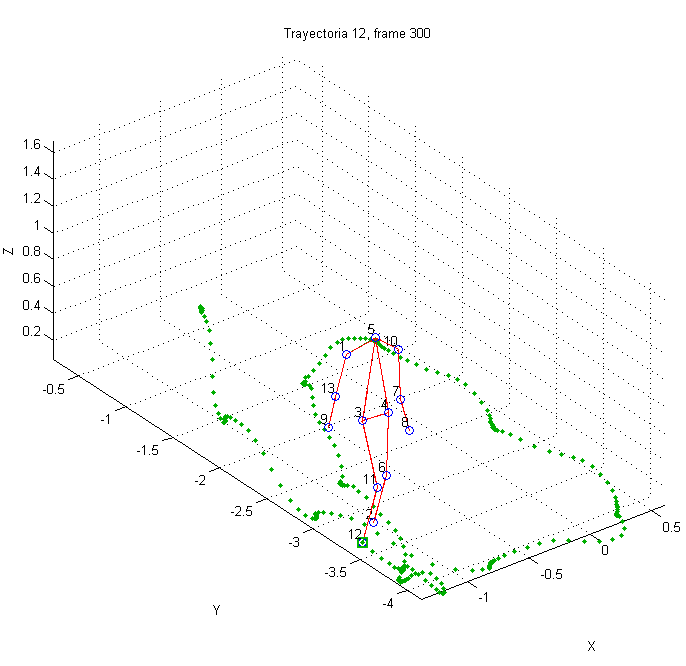
\includegraphics[scale=0.4]{img/Performance/00_Animacion_Tracking.png}}  
   \caption{Trayectorias obtenidas para Movimiento Libre.}
  \label{captura_movimiento_libre}
\end{figure} 

\begin{table}[h]
\centering
\begin{tabular}{c|c|c|c|c|c|}
\cline{2-6}
\textbf{} & \textbf{CONJUNTO} & \multicolumn{2}{c|}{\textbf{C15}} & \multicolumn{2}{c|}{\textbf{C8}} \\ \hline
\multicolumn{1}{|c|}{\textbf{NUMERO}} & \textbf{NOMBRE} & \textbf{\begin{tabular}[c]{@{}c@{}}Promedio\\ (cm)\end{tabular}} & \textbf{\begin{tabular}[c]{@{}c@{}}99\%\\ (cm)\end{tabular}} & \textbf{\begin{tabular}[c]{@{}c@{}}Promedio\\ (cm)\end{tabular}} & \textbf{\begin{tabular}[c]{@{}c@{}}99\%\\ (cm)\end{tabular}} \\ \hline
\multicolumn{1}{|c|}{1} & LeftUpLeg & 0,4695 & 2,7781 & 0,4232 & 1,2907 \\ \hline
\multicolumn{1}{|c|}{2} & LeftLeg & 0,4176 & 1,4028 & 0,4232 & 2,3317 \\ \hline
\multicolumn{1}{|c|}{3} & LeftFoot & 0,3935 & 0,714 & 0,4045 & 0,6123 \\ \hline
\multicolumn{1}{|c|}{4} & RightUpLeg & 0,4451 & 2,9214 & 0,3882 & 1,4679 \\ \hline
\multicolumn{1}{|c|}{5} & RightLeg & 0,3726 & 1,0633 & 0,3475 & 0,7875 \\ \hline
\multicolumn{1}{|c|}{6} & RightFoot & 0,3633 & 0,8745 & 0,3858 & 2,204 \\ \hline
\multicolumn{1}{|c|}{7} & Head & 0,4068 & 1,5204 & 0,369 & 0,5278 \\ \hline
\multicolumn{1}{|c|}{8} & LeftArm & 0,3951 & 0,7051 & 0,4139 & 1,4362 \\ \hline
\multicolumn{1}{|c|}{9} & LeftForeArm & 0,467 & 2,9049 & 0,3852 & 0,5232 \\ \hline
\multicolumn{1}{|c|}{10} & LeftHand & 0,4259 & 1,5519 & 0,3923 & 0,5664 \\ \hline
\multicolumn{1}{|c|}{11} & RightArm & 0,3845 & 0,8526 & 0,4395 & 1,7055 \\ \hline
\multicolumn{1}{|c|}{12} & RightForeArm & 0,3987 & 1,696 & 0,3441 & 0,5617 \\ \hline
\multicolumn{1}{|c|}{13} & RightHand & 0,3866 & 1,1216 & 0,3528 & 0,7263 \\ \hline
 & \textbf{Secuencia} & \textbf{0,39741} & \textbf{1,4952} & \textbf{0,37824} & \textbf{1,2867} \\ \cline{2-6} 
\end{tabular}
\end{table}

\begin{table}[h]
\centering
\begin{tabular}{c|c|c|c|c|c|}
\cline{2-6}
\textbf{} & \textbf{CONJUNTO} & \multicolumn{2}{c|}{\textbf{C6.3}} & \multicolumn{2}{c|}{\textbf{C4.2}} \\ \hline
\multicolumn{1}{|c|}{\textbf{NUMERO}} & \textbf{NOMBRE} & \textbf{\begin{tabular}[c]{@{}c@{}}Promedio\\ (cm)\end{tabular}} & \textbf{\begin{tabular}[c]{@{}c@{}}99\%\\ (cm)\end{tabular}} & \textbf{\begin{tabular}[c]{@{}c@{}}Promedio\\ (cm)\end{tabular}} & \textbf{\begin{tabular}[c]{@{}c@{}}99\%\\ (cm)\end{tabular}} \\ \hline
\multicolumn{1}{|c|}{1} & LeftUpLeg & 0,8081 & 9,8783 & 3,9761 & 23,5115 \\ \hline
\multicolumn{1}{|c|}{2} & LeftLeg & 0,5145 & 3,5296 & 0,959 & 9,4765 \\ \hline
\multicolumn{1}{|c|}{3} & LeftFoot & 0,4198 & 0,6535 & 0,9796 & 17,8756 \\ \hline
\multicolumn{1}{|c|}{4} & RightUpLeg & 0,4243 & 2,0492 & 6,5918 & 36,9034 \\ \hline
\multicolumn{1}{|c|}{5} & RightLeg & 0,3553 & 1,0051 & 0,8372 & 15,4254 \\ \hline
\multicolumn{1}{|c|}{6} & RightFoot & 0,3852 & 2,2009 & 1,1164 & 30,4735 \\ \hline
\multicolumn{1}{|c|}{7} & Head & 0,3803 & 0,5388 & 0,378 & 0,526 \\ \hline
\multicolumn{1}{|c|}{8} & LeftArm & 0,4288 & 1,3562 & 1,5435 & 20,0225 \\ \hline
\multicolumn{1}{|c|}{9} & LeftForeArm & 0,3955 & 0,5965 & 0,8621 & 12,847 \\ \hline
\multicolumn{1}{|c|}{10} & LeftHand & 0,398 & 0,5513 & 1,5922 & 17,1708 \\ \hline
\multicolumn{1}{|c|}{11} & RightArm & 0,5743 & 3,208 & 5,5887 & 25,7882 \\ \hline
\multicolumn{1}{|c|}{12} & RightForeArm & 0,358 & 0,6621 & PERDIDO & PERDIDO \\ \hline
\multicolumn{1}{|c|}{13} & RightHand & 0,3492 & 0,6748 & PERDIDO & PERDIDO \\ \hline
 & \textbf{Secuencia} & \textbf{0,43212} & \textbf{2,4391} & \textbf{1,8061} & \textbf{25,7332} \\ \cline{2-6} 
\end{tabular}
\end{table}

\end{itemize}

Comportamiento caso real?


